El enfoque de la aplicación en assembler era poder procesar 16 bytes contiguos con instrucciones simultaneas para poder aprovechar al máximo el paralelismo que ofrece SIMD. Esto no fue posible debido a que el set de instrucciones no tiene comparaciones de greater, lower o derivadas para bytes sin signo (necesario ya que los pixeles en grayscale van del 0 al 255) por lo que fué necesario realizar un desempaquetamiento de los datos (convirtiendolos en words) y se consiguió operar sobre los bytes de a 8 por instrucción SIMD, aunque por cada ciclo se lograron procesar los 16.

Para optimizar el procesamiento dentro del ciclo, se calcula y se guarda en registros xmm al inicio del programa:
\begin{itemize}
  \item xmm12 $\Rightarrow$ Contiene 16 bytes packed con el mínimo
  \item xmm11 $\Rightarrow$ Contiene el mínimo packed en words
  \item xmm5 $\Rightarrow$ Contiene el máximo packed en words
  \item xmm6 $\Rightarrow$ Contiene la representación flotante de Q packed
\end{itemize}

\subsubsection{Descripción del ciclo:}
Al comienzo del ciclo se ponen en 0 los bytes del registro xmm8 que servirá como acumulador de los nuevos valores que tendrán los pixeles.

Se guardan 16 bytes contiguos desde la imagen fuente en el registro xmm1, se busca cuáles son iguales al mínimo (aprovechando la instrucción pcmpeqb que realiza la comparación en los 16 bytes simultaneamente) y se guarda la máscara obtenida que se usará mas tarde. Luego se los desempaqueta en parte alta y baja extendiendolos a words para realizar comparaciones.

\begin{figure}[ht!]
\centering
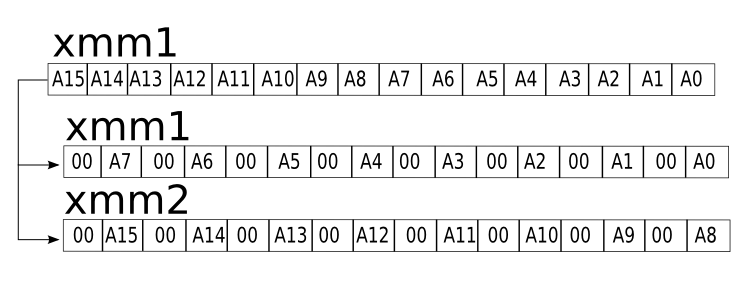
\includegraphics[width=90mm]{unpackxmm1.png}
\caption{Desempaquetado de los bytes a words para realizar comparaciones}
\label{overflow}
\end{figure}

Se buscan los números que superen al máximo comparando la parte alta y baja con el registro xmm5 preparado al inicio del programa el cuál contiene el máximo en words empaquetadas. Utilizando pcmpgtw tanto en la parte baja como la alta, obtenemos una máscara que contiene en 0xFFFF las words mayores al máximo y en 0x0000 las demás. Empaquetamos la máscara relacionada a la parte baja y a la alta dejando en 255 sólo los bytes que sean mayores al máximo para luego sumarlos en el acumulador.


\begin{figure}[ht!]
\centering
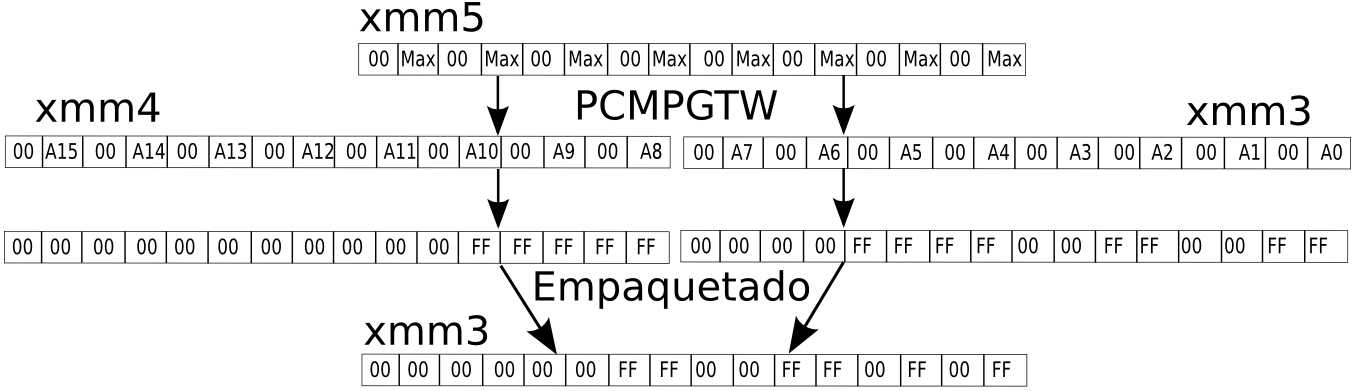
\includegraphics[width=150mm, height=40mm]{cpmmax.png}
\caption{Ejemplo de creación de máscara y empaquetado de la misma. El registro xmm3 es la copia de xmm1 que guardará la parte baja de la máscara, xmm4 realiza lo mismo con la parte alta.}
\label{overflow}
\end{figure}

Al utilizar un acumulador incialmente en 0 se pudo ahorrar el paso de comparar los pixeles menores al mínimo ya que los pixeles que cumplieran esta propiedad tendrían 0 como valor.

Para conseguir la máscara para el caso en el que el valor del pixel estuviera entre el máximo y el mínimo ($min \geq p \leq max$) se aprovechó las máscaras previamente obtenidas (mayores al máximo e iguales al mínimo), por lo que sólo fue necesario buscar los números mayores al mínimo (haciendo un procedimiento similar al de la búsqueda del máximo), agregarle los números iguales al mínimo (mediante un por) con la máscara creada al principio del ciclo y luego sacarle los mayores al máximo (mediante un pxor).

Luego de haber creado la máscara para el caso, se realiza el cálculo de los nuevos valores para los pixeles que cumplan esa propiedad, los cuales deben realizarse utilizandose punto flotante. Fue necesario desempaquetar aún más los pixeles para poder obtener los valores de estos en double words y poder convertirlos a single precision floats, precisión suficiente para los cálculos que también brinda la posibilidad realizar más operaciones sobre los pixeles simultanteamente que con doubles.

Se realiza el desempaquetado de la parte baja anteriormente desempaquetada (xmm1) y se los convierte a single presicion floats. Luego se los divide por el registro xmm6 el cuál contiene el valor Q empaquetado en single presicion floats calculado al inicio del programa. Se lo trunca para realizar la función "floor" convirtiendose en entero, se lo convierte otra vez a float y se lo termina multiplicando por xmm6 otra vez para finalmente ser convertido a entero, obteniendo el valor correspondiente para cáda pixel. Se vuelve a empaquetar obteniendose otra vez los valores nuevos de los pixeles en words y se repite la operación con la parte alta del desempaquetamiento inicial (xmm2).

Al finalizar, se empaquetan los dos registros resultantes para luego poder aplicarle la máscara anteriormente creada para el caso y sumar el valor obtenido al acumulador, dejando el valor correspondiente en los pixeles que cumplían con el caso.

Por último, se copian los nuevos valores de los 16 bytes en la imagen destino, se incrementan los punteros de la imágen fuente y destino para la próxima iteración. También se resta nuestro contador de pixeles, se lo compara para ver si llegó al final, caso en el que termina la ejecución, o si quedan más e igual, caso en el que vuelve a ciclar, o si restan menos de 16 bytes por agarrar, dónde se vuelve para atrás los punteros de las imágenes para que queden 16 pixeles exactamente y se pueda realizar la última iteración.



\subsubsection{Discusión y comparación con el código C:}
Enfocandonos en la versión decompilada de umbralizar\_c.c utilizando objdump -d -M intel -S umbralizar\_c.o se pueden observar bien en detalle las instrucciones que utiliza el compilador para ensamblar la versión en c de umbralizar.

Se puede observar que el compilador, al tratarse del lenguaje C y su convención utiliza el stack para guardar variables locales, algo que seguramente será cubierto por la memoria caché pero que es comparable contra utilizar casi únicamente registros, que otorgan mejor performance a la hora de utilizar datos, como se realiza en la implementación en assembler.

Enfocandonos un poco en los condicionales, se puede ver como la versión en c desensamblada produce el código respectivo para calcular la posición del byte específico a comparar en la matríz fuente cada vez que se quiere realizar la comparación. La eficiencia de la implementación en c es muy evidente, no sólo no es necesario calcular la posición ya que se toman 16 bytes contiguos en vez de la utilización del casteo matricial, si no que las comparaciones se realizan en simultaneo. Si bien se comparan y se procesan 8 bytes por instrucción ya que es necesario extenderlas y compararlas de a 8, en cada ciclo del algoritmo se procesan 16 bytes. Cuándo se habla de procesar, se tiene en cuenta las operaciones tanto de comparación como de cálculo para los valores resultantes de los píxeles. También queda en evidencia que el algoritmo programado en assembler hace sólo dos llamadas a memoria, una para traer los 16 bytes contiguos y otra para modificar estos 16 bytes por sus correspondientes valores, algo muy superior a pedir y modificar bytes de a uno (VER EJEMPLO TIEMPO).

Por el lado del cálculo de $floor(ecuacion) * q$ dónde $ecuacion = src_matrix[y][x] / q$ , las operaciones de punto flotante se realizan con escalares, de a una en cada iteración por el lado de c, mientras que la implementación en assembler contempla operaciones simultaneas para estas.